\documentclass[
    iai, % Saisir le nom de l'institut rattaché
    il, % Saisir le nom de l'orientation
]{heig-tb}

\usepackage[nooldvoltagedirection,european,americaninductors]{circuitikz}
\usepackage{graphicx}
\graphicspath{ {./assets/img/} }

\signature{signature.svg}

\makenomenclature
\makenoidxglossaries
\makeindex

\addbibresource{bibliography.bib}

\usepackage{etoolbox}
\renewcommand\nomgroup[1]{%
  \item[\bfseries
  \ifstrequal{#1}{A}{Constantes physiques}{%
  \ifstrequal{#1}{B}{Groupes}{%
  \ifstrequal{#1}{C}{Autres Symboles}{}}}%
]}

\newcommand{\nomunit}[1]{%
\renewcommand{\nomentryend}{\hspace*{\fill}#1}}

\nomenclature[A, 02]{\(c\)}{\href{https://physics.nist.gov/cgi-bin/cuu/Value?c}
{Vitesse de la lumière dans le vide}
\nomunit{\SI{299792458}{\meter\per\second}}}

\nomenclature[A, 03]{\(h\)}{\href{https://physics.nist.gov/cgi-bin/cuu/Value?h}
{Constante de Planck}
\nomunit{\SI[group-digits=false]{6.62607015e-34}{\joule\per\hertz}}}

\nomenclature[A, 01]{\(G\)}{\href{https://physics.nist.gov/cgi-bin/cuu/Value?bg}
{Constante de gravitation universelle}
\nomunit{\SI[group-digits=false]{6.67430e-11}{\meter\cubed\per\kilogram\per\second\squared}}}

\nomenclature[B, 03]{\(\mathbb{R}\)}{Nombres réels}
\nomenclature[B, 02]{\(\mathbb{C}\)}{Nombres complexes}
\nomenclature[B, 01]{\(\mathbb{H}\)}{Quaternions}

\nomenclature[C]{\(V\)}{Volume constant}
\nomenclature[C]{\(\rho\)}{Indice de frottement sec}

\newacronym{gcd}{GCD}{Plus grand diviseur commun}
\newacronym{lcm}{LCM}{Plus petit multiple commun}

\newglossaryentry{heig-vd}{
    name=HEIG-VD,
    description={Haute École d'Ingénierie et de Gestion du canton de Vaud}
}

\newglossaryentry{uml}{
    name=UML,
    description={Notation pour la modélisation d'applications en ingénieurie logiciel}
}

\newglossaryentry{diagrams}{
    name=diagrams.net,
    description={Site web permettant de créer des diagrammes}
}

\newglossaryentry{websig}{
    name=webSIG,
    description={systèmes d'interface web de visualisation de données géographiques}
}

\newglossaryentry{epfl}{
name=EPFL
description={Ecole polytechnique fédéral de Lausanne}
}
% Auteur du document (étudiant-e) en projet de Bachelor
\author{Kylian Bourcoud}

% Activer l'option pour l'accord du féminin dans le texte
%\genre{female}

% Titre de votre travail de Bachelor
\title{Plans de la HEIG-VD interactifs}

% Le sous titre est optionnel
\subtitle{Travail de Bachelor}

% Nom du professeur responsable
\teacher {Prof. Y. Chevallier (HEIG-VD)}

% Mettre à jour avec la date de rendu du travail
\date{\today}

% Numéro de TB
\thesis{7212}



\surroundwithmdframed{minted}

%% Début du document
\begin{document}
\selectlanguage{french}
\maketitle
\frontmatter
\clearemptydoublepage

%% Requis par les dispositions générales des travaux de Bachelor
\preamble
\authentification

%% Résumé / Version abbrégée
\begin{abstract}
    % Francais
Ce rapport décrit le processus de création d'une application web de plans interactifs pour la HEIG-VD.
Ce processus est séparé en cinq étape : une introduction au contexte,
une analyse des besoins des utilisateurs et des sytèmes déja existentes,
la conception d'une solution, la réalisation de celle-ci,
et finalement une critique du travail accompli.



\asterism

% English
This report describes the creation process for a web application of interactive plan for the HEIG-VD school.
This process is separated in five steps : an introduction of the context,
an analysis of the users needs and the existants solutions,
the conception of a solution, the development
and finally a review of the accomplished work.
\end{abstract}

%% Sommaire et tables
\clearemptydoublepage
{
    \tableofcontents
    \let\cleardoublepage\clearpage
    \listoffigures
    \let\cleardoublepage\clearpage
    \listoftables
    %\let\cleardoublepage\clearpage
    %\listoflistings
}

\printnomenclature
\clearemptydoublepage
\pagenumbering{arabic}

%% Contenu
\mainmatter
\chapter{Introduction}
\section{Contexte}
Les cartes qu'elle soit schématique ou précise ont été un outil très utile pour l'orientation des personnes au sein d'une région ou d'un bâtiment.
Avec l'arrivée du web, l'usage des plateformes de cartes comme google maps ont peu à peu remplacer les cartes papier, amenant des fonctionnalités plus interactives.

\begin{figure}[H]
    \centering
    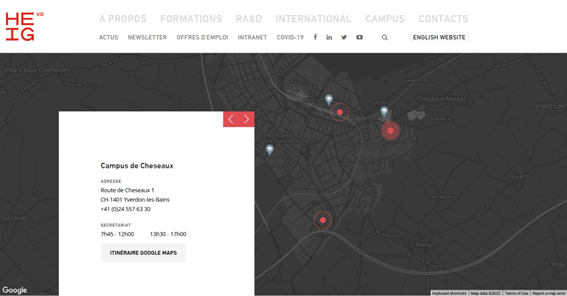
\includegraphics{actual_heig_plan.png}
    \caption{Plans actuels de la HEIG-VD}
    \label{fig:heigCurrentMap}
\end{figure}
La \gls{heig-vd} est une haute école dispensant des formations dans différents domaines de l'ingénieurie, ainsi que de la gestion d'entreprise.
Elle se situe sur trois sites dispersé dans la ville d'Yverdon-Les-Bains
: Cheseaux  situé en périphérie de la ville, St-Roch situé proche de la gare et le Y-Parc situé dans la zone industrielle.

Cette école fournit, sur son site web un plan \cite{plan-heig} (voir Figure \ref{heigCurrentMap}) indiquant l'emplacement des trois bâtiments pricipaux.
On peut aussi y obtenir les informations sur les différents moyens d'accès à ces sites afin d'aider ses utilisateurs à s'orienter.
Cependant elle ne fournit, ni sur son site, ni dans le guide de l'étudiant, une interface permettant de s'orienter vers une salle ou une ressource précise.

\section{Description du problème}
M.Chevallier souhaite mettre à disposition aux utilisateurs une interface interactive pour visualiser les salles et les plans de la \gls{heig-vd} pour les trois bâtiments.

\chapter{Analyse}
\section{Analyse fonctionnelle du système}
L'analyse fonctionnelle est un processus qui permets de déterminer les fonctionnalités d'un système à partir d'une analyse des besoins utilisateurs.

\subsection{Cas d'utilisation}
La première étape est de déterminer les cas d'utilisations du futur système.
Ceux-ci ont été établi lors de la conception du schéma des cas d'utilisation, figure \ref{useCaseDiagram.xml}.
Celui-ci est en notation \gls{uml}, un des standards utilisé dans la modélisation d'application logiciel,
et a été réalisé à l'aide de l'application web \gls{diagrams} \cite{diagrams}.

\fig[width=9cm]{Schéma des cas d'utilisations}{useCaseDiagram.drawio.pdf}

\newpage
Ce schéma présente les cas d'utilisation suivant :
\begin{itemize}
    \item Un utilisateur utilise le système pour s'orienter sur les différents sites de la HEIG-VD.
    \item Un utilisateur opère une recherche sur le système afin de localiser une ressource par des critères ou par son nom (une ressource est un terme générique pouvant symboliser une salle, l'emplacement d'un bureau d'un collaborateur, l'emplacement de matériel, etc.).
    \item Un utilisateur obtient des informations sur une ressource.
    \item Un utilisateur personnalise la carte et l'exporte pour d'autre usage.
\end{itemize}

\subsection{Analyse des besoins}
La deuxième étape de l'analyse fonctionnelle est de déterminer les besoins des utilisateurs à partir des cas d'utilisation du système.
Pour ce système les besoins ont été déterminé dans le tableau \ref{besoins}. Ils ont été numérotés de N1 à N8 pour pouvoir s'y référer plus facilement par la suite.
\begin{table}[H]
    \begin{center}
        \caption{Liste des Besoins \label{besoins}}
        \begin{tabular}{l|l}
               & Besoin                                                                  \\ \hline
            N1 & S'orienter facilement à travers les sites de la HEIG-VD                 \\
            N2 & Localiser une ressource à l'aide de son nom                             \\
            N3 & Localiser une ressource à l'aide de critères                            \\
            N4 & S'informer efficacement sur une ressource                               \\
            N5 & Être capable de personnaliser une carte                                 \\
            N6 & Être capable de partager sa carte personnalisée                         \\
            N7 & S'informer efficacement des noms des locaux, leur surface, et leur type \\
            N8 & Localiser facilement un collaborateur sur un plan des sites
        \end{tabular}
    \end{center}
\end{table}

\newpage

\subsection{fonctionnalités du système}
La troisième étape est de déterminer les fonctionnalités du système à partir des besoins des utilisateurs.
Ils ont été listés dans le tableau ci-dessous.
De plus les besoins auxquelles ils répondent, ont été précisé dans la troisième colonne du tableau.
\begin{table}[H]
    \begin{center}
        \caption{Liste des Fonctionnalités \label{fonctions}}
        \begin{tabular}{l|l|l}
                & fonctionnalités                                                      & besoin   \\ \hline
            F1  & Afficher un plan afin d'aider l'orientation                          & N1 N7    \\
            F2  & Utilisable facilement et de façon ergonomique                        & N1       \\
            F3  & Fournir une orientation rapidement                                   & N1       \\
            F4  & Facilement accessible                                                & N1       \\
            F5  & Afficher les ressources désirées                                     & N1 N3 N5 \\
            F6  & Fournir un outil de tracé de plus cour itinéraire pour l'orientation & N1       \\
            F7  & Offrir un outil de localisation de ressource par nom                 & N2 N8    \\
            F8  & Fournir un outil de localisation de ressource par critères           & N3       \\
            F9  & Fournir des informations sur les ressources                          & N4 N7    \\
            F10 & Fournir un outil de dessin sur carte                                 & N5       \\
            F11 & Fournir un outil d'exportation                                       & N5       \\
            F12 & Fournir un outil d'impression de carte                               & N6       \\
            F13 & Fournir un outil de partage de carte                                 & N6       \\
            F14 & Fournir un outil de sauvegarde de carte                              & N6
        \end{tabular}
    \end{center}
\end{table}

\section{Etat de l'art des systèmes d'informations géographiques}
Avant de commencer un projet, il est important de connaître ce qui a déjà été fait dans le domaine et les ressources à notre disposition.
Dans ce chapitre, je vais, analyser différents systèmes d'interface de plans interactifs,
les technologies utilisé pour aider la construction d'un logiciel Web GIS et les ressources que j'ai à disposition.

\subsection{Systèmes existants d'interface interactive}

\subsection{Plan EPFL}
\begin{figure}[H]
    \caption{Plans interactifs de l'EPFL}
    \centering
    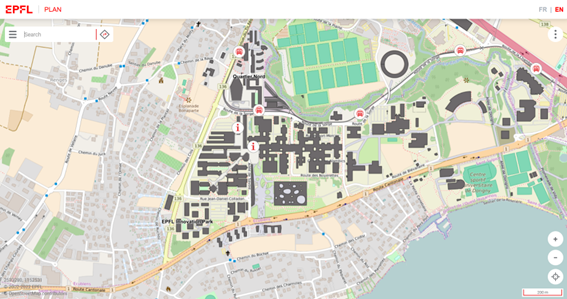
\includegraphics{planEPFL.png}
\end{figure}

\textbf{Fonctionnalités}

Les plans interactifs du campus de l'EPFL \cite{plan-epfl} affichent les bâtiments du campus en s'adaptant selon le zoom et l'étage sélectionné.
Suivant le zoom on peut visualiser le contour du site, puis les le contour des bâtiments et enfin les salles des bâtiments.

\begin{figure}[H]
    \caption{Zoom sur les plans de l'EPFL }
    \centering
    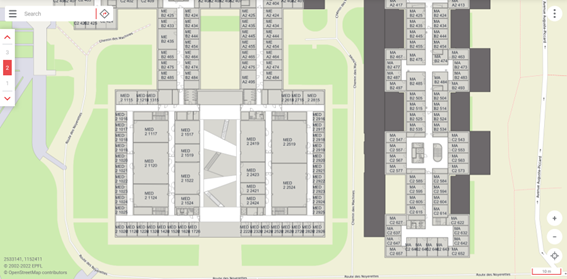
\includegraphics{planEPFLGrosPlan.png}
\end{figure}

L'utilisateur a la possibilité de filtrer les points d'intérêts à afficher sur la carte à l'aide d'un menu sur la gauche du site.
Il y a aussi la possibilité de rechercher différentes ressources en fonction de leur nom comme les bâtiments, les salles, les personnes, les restaurant, les magasins, ou encore les espaces culturels.
D'autre outil sont fournis comme la recherche d'un plus court itinéraire entre deux ressources, un outil pour l'impression, changer l'affichage pour une vue aérienne.
Finalement un lien permet d'accéder au Géoportail de l'EPFL.

\textbf{Technologies utilisées}

La principale technologie utilisée pour le frontend est Ngeo (combine Angular js et openlayers, plus de détails dans la section technologie ).

\subsection{Géoportail EPFL}

\begin{figure}[H]
    \caption{Géoportail de L'EPFL}
    \centering
    \includegraphics{géoportailEPFL.png}
\end{figure}

Le Géoportail de l'EPFL \cite{geoportail-epfl} est très similaire au plan du campus, mais il offre la possibilité de dessiner des formes vectorielles sur la carte.
Il permet aussi d'afficher des ressources plus précises comme les réseaux wifi ou les prises électrique.

\subsection{MIT campus map}

\begin{figure}[H]
    \caption{carte du campus du MIT}
    \centering
    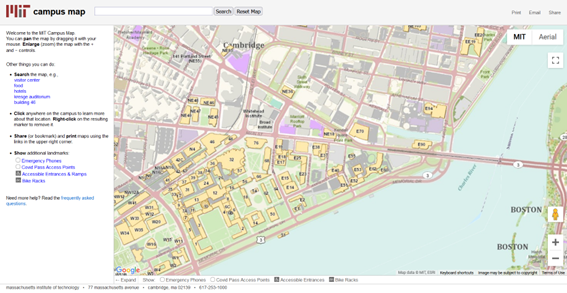
\includegraphics{MitCampusMap.png}
\end{figure}

\textbf{Fonctionnalités}

Le plan interactif du MIT \cite{mit-map} affiche le tracé des bâtiments ainsi que le nom de ceux-ci. Seulement les légendes s'adaptent en fonction du zoom.

Un utilisateur peut rechercher des bâtiments ou des points d'intérêts lié à l'université (ex : le world wide web consortium W3C).

Il peut aussi appliquer quelques filtres pour afficher des repères comme les restaurants. Cliquer sur un bâtiment permet d'obtenir des informations sur celui-ci. D'autres outils sont fournis comme un outil de partage ou d'impressions.

\textbf{Technologies utilisées}

L'affichage de la carte s'effectue à l'aide de l'api google maps. Ceci permet aussi un accès à google street view.

\subsection{SITN - Géoportail du système d'informations du territoire neuchâtelois}

\begin{figure}[H]
    \caption{Plan du SITN}
    \centering
    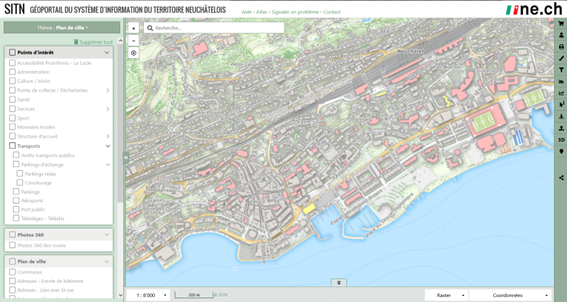
\includegraphics{planSITN.png}
\end{figure}

\textbf{Fonctionnalités}

Les plans du SITN \cite{sitn} affichent les différentes informations géographiques du canton de Neuchâtel.
Le niveau de détail de la carte s'adapte en fonction du zoom.
Par exemple les numéros des maisons selon le cadastre de chaque commune s'affichent lors d'un zoom à une échelle 1 :1000.

Il y a la possibilité d'appliquer plusieurs filtres afin d'obtenir les informations recherchées comme le tracé des commune ou les points d'intérêts.

L'outil offre aussi des outils de dessin vectoriel, d'impression, la possibilité de changer le fond du plan de changer un accès à google street map, et un accès au géoportail LIDAR

\textbf{Technologies utilisées}

Le site utilise GeoMapfish pour l'affichage des cartes ainsi que l'api google maps pour google street view.

\subsection{Standford Campus Map}

\begin{figure}[H]
    \caption{plan du campus de Standford}
    \centering
    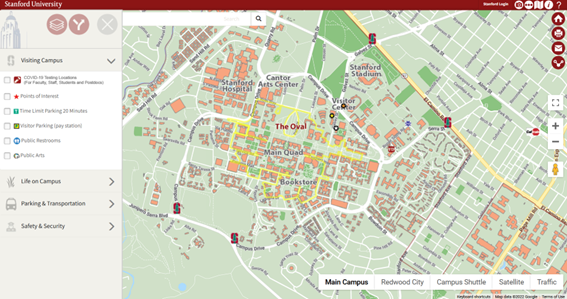
\includegraphics{standfordCampusMap.png}
\end{figure}

\textbf{Fonctionnalités}

Le carte du campus de Standford \cite{standford-map} affiche le tracé des bâtiments ainsi qu'une légende précisant le nom de ceux-ci.
Seul l'affichage de la légende varie selon le zoom : affiche seulement les légendes lors d'un affichage rapproché sur les bâtiments.

Le site offre un outil de recherche de ressources aux utilisateurs, un accès à open street view, un outil d'impression et un outil de partages.

A noter que le menu en bas à droite est un mélange de plusieurs fonctionnalités ce qui peut perdre un nouvel utilisateur.

\textbf{Technologies utilisées}

L'application web utilise l'api google maps pour l'affichage de la carte.

\subsection{Aéroport de Zürich}

\begin{figure}[H]
    \caption{Plan de l'aéroport de Zürich}
    \centering
    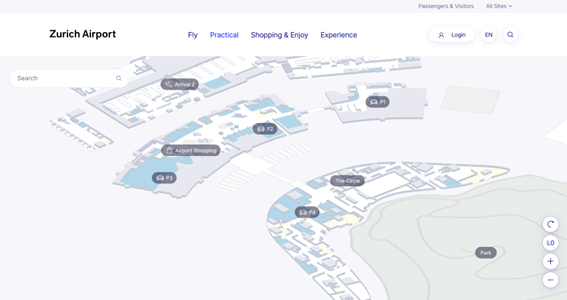
\includegraphics{planZurichAirport.png}
\end{figure}

\textbf{Fonctionnalités}

L'aéroport de Zurich \cite{zurich-aeroport} offre un plan non géoréférencé en 3d isométrique.
Les différents points d'intérêts affichés varient en fonction du zoom.
L'application offre un outil de recherche avec des suggestions par thème.
On peut aussi changer le fond du plan en fonction de l'étage.

Le plan ne sert que pour l'orientation des voyageurs et est donc pauvre en fonctionnalité annexe.

\textbf{Technologies utilisées}
Le site utilise le Framework réactif React js, ainsi que le module bundler webpack.  Les plans sont des images bitmap (pixellisé).

\subsection{Conclusion de l'analyse des systèmes existants}
On peut distinguer deux types d'application :
des plans interactifs qui aides des utilisateurs à s'orienter et les Géoportails qui fournissent des informations géographiques et permet de construire de nouvelles informations à l'aide d'outils de dessin vectoriel.

Cette distinction a été faite par l'EPFL, qui sépare sur deux sous-domaines différents, les deux types d'application.

Les technologies utilisées sont aussi différentes : les sites les plus complets utilisent souvent geomapfish alors que les sites les plus simples utilisent plutôt l'api google maps.

\section{Architecture WebGIS}

\begin{figure}[H]
    \caption{Architecture classique d'une infrastructure WebGIS}
    \centering
    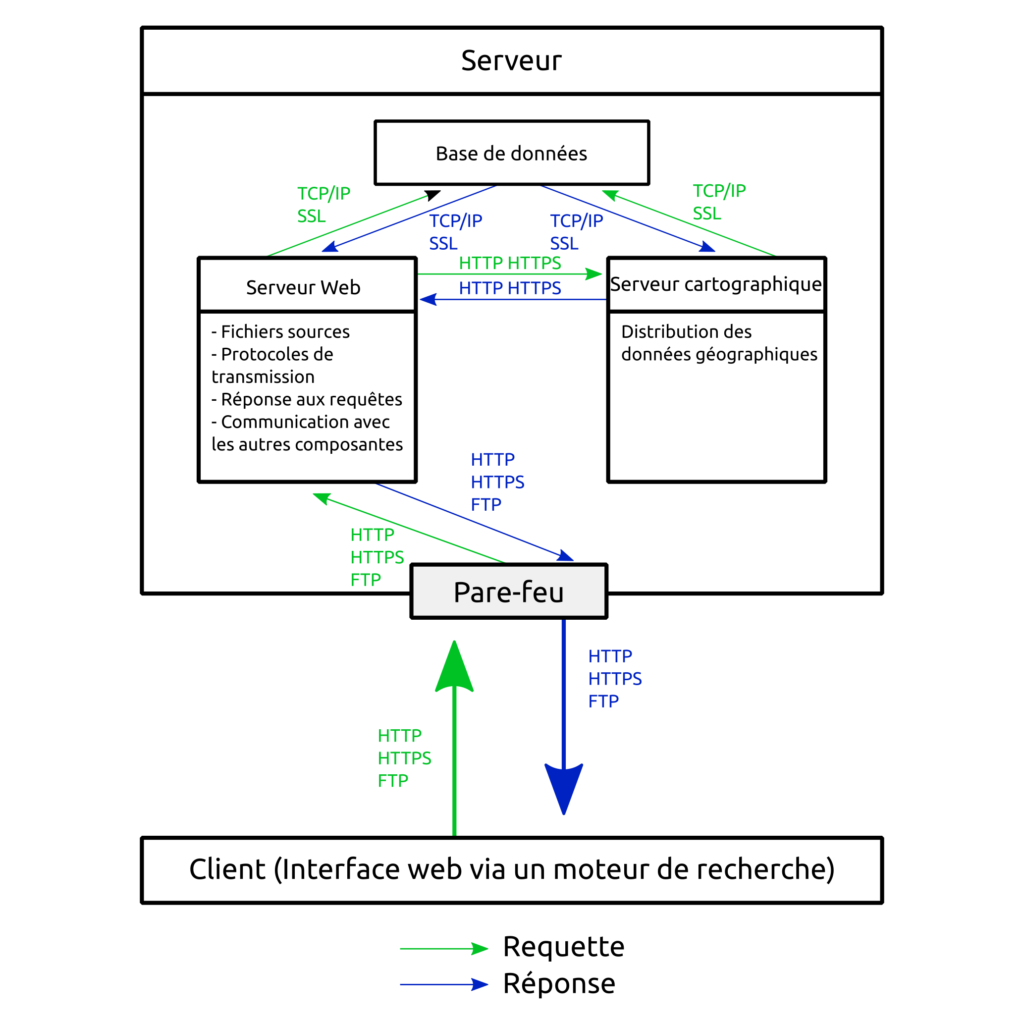
\includegraphics[scale=0.3]{webGIS_archi.png}
\end{figure}

Une application webGIS \cite{architecture-webgis} est composée, côté serveur, d'une base de données stockant les données géographiques, et un serveur cartographique qui gère et distribue les données géographiques.
La distribution se fait à l'aide des protocoles WMS/WMTS/WFS.
Finalement un serveur web envoie la page et les données géographique au client.

\section{Technologies }

\subsection{Openlayers}
Openlayer \cite{openlayers} est une librairie JavaScript open source qui facilite la construction d'appllication webGIS.
Elle permet de rajouter facilement des calques contenant des données géographiques en dessus d'un fond de carte.
Elle peut lire plusieurs formats de données comme du geojson ou du KML.

\subsection{Leaflet}

Leaflet \cite{leaflet} est une librairie open source concurrente à openlayers.
Elle est plus simple d'utilisation et légère mais moins complète que openlayers.
On peut rajouter des plugins à la librairie.

\subsection{Google maps API}
L'API de google maps \cite{google-maps} n'est pas open source et peut être payant.
Elle n'offre pas la possibilité de rajouter des calques au fond de carte, seulement des points d'intérêts.

\subsection{GeoMapfish}
GeoMapFish est une technologie open source développé par camptocamp et permet de faciliter la construction de système d'information géographique pour le web (webGIS).
Il est composé de Ngeo pour le frontend \cite{ngeo} et de c2cgeoportal \cite{c2cgeoportal} pour le backend.

Ngeo est une librairie JavaScript qui facilite le développement d'application basé sur le Framework réactif Angular Js et l'api openLayers.
Elle utilise aussi webpack comme module bundler.

C2cGeoportal est la partie serveur construit à partir d'une image Docker. Il faut avoir une connaissance en Python pour l'utiliser.

\subsection{Serveur cartographique}
Qgis server \cite{qgis} est un serveur cartographique open source gérant les protocoles WMS WFS et WCS écrit en c++.

ArcGIS server \cite{arcgis} est un composant de la suite ArcGIS entreprise. Ce logiciel est propriétaire et payant.

Geoserver \cite{geoserver} est un serveur cartographique open source écrit en java. Il intègre la librairie openlayers.

Mapserver \cite{mapserver} est le premier serveur cartographique. Il supporte les protocoles WMS WFS et WCS.

\subsection{PostGreSQL et PostGis}
PostGreSQL est une base de données relationnelle open source, elle permet de stocker des données géographiques avec l'extension PostGis  \cite{postgis}.
Cette solution est utilisée par c2cgeoportal.

\section{Données existantes à disposition}
\subsection{Plans}
Des plans des étages des sites de Cheseaux et St-Roch non géoréférencé m'ont été fournis au format DGW, format propriétaire de AutoCAD.
Il faudra les géoréférencé à l'aide d'un logiciel GIS dans une projection compatible avec les technologies choisis à l'aide d'une transformation de Helmert.

\subsection{Serveur LDAP}
Le serveur LDAP de la HEIG-VD peut fournir des informations sur certaines ressources.




\chapter{Conception de la solution}
\section{Exigences de la solution}
Il a été établi que je mettrai en place une interface interactive de visualisations des plans comprenant uniquement le site de Cheseaux.
Celui-ci devra afficher toute les salles du site avec leurs noms, un qualificatif (Secrétariat, salle de cours, etc.) et leur surface en mètres carrés.
Un outil de changement d'étage permettra de parcourir les différents étages du site.
L'interface sera disponible autant sur de grands écrans comme une télévision que sur de petits écrans comme les téléphones mobiles

Cette application sera hébergée sur une machine virtuel fournit par l'école.
Elle comportera une base de données qui s'occupera de stocker les données utilisées.
Un serveur API récupérera les données et les enverra a l'utilisateur.

Elle positionnera aussi certaines ressources comme les collaborateurs sur le site de la HEIG-VD.

Si le temps le permet, un outil de filtrage des ressources à affichés et/ou un outil de recherche sera aussi développé.

\section{Infrastructure}

\figi{infra.xml}{9cm}{Architecture de l'infrastructure}

Lorsqu'il va accéder à l'application, l'utilisateur va demander les différents fichiers HTML, CSS et Javascript à un petit serveur.
Ce serveur aura été développé en JavaScript grâce à node JS.
Il utilisera le Framework web express JS, car celui-ci est léger et minimaliste, le serveur ne nécessitant pas beaucoup de développement.

Par la suite, en fonction des manipulations de l'utilisateurs, l'application va demander des données à un serveur API.
Par exemple, lorsque l'utilisateur veut afficher un étage, l'application va demander les données nécessaire pour l'affichage de ce nouvel étage.
Le serveur API sera aussi développé en javascript à l'aide de node JS. Cependant il utilisera le Framework web Nest Js.
Celui-ci est beaucoup plus complet par rapport à express JS. Il est utile car le serveur nécessite une connexion à la base de données.

Finalement l'infrastructure est composée d'une base de données relationnelle PostGreSQL.
Celle-ci est étendu par l'extension PostGis qui permet le stockage de données géographiques.

\section{Pipeline CI/CD}

\figi{pipeline.xml}{12cm}{Pipeline CI/CD}

Le système sera composé à la base de trois applications node JS :
Un frontend qui construira les pages HTML, CSS et JavaScript à l'aide du Framework Angular JS et de Webpack.
La librairie NGeo permettra l'affichage des plans interactifs.

Un petit serveur développé à l'aide du Framework expressJS qui aura pour but après déploiement de fournir les fichiers statiques compilés par le frontend.

Un serveur API développé à l'aide du Framework NestJs qui aura pour but de récupérer les données depuis de la base de données et les envoyer à l'application web.

Les codes sources seront hébergé sur le service Gitlab. Il sera composé de deux branches :
une branche main qui hébergera le code source destiné à la production et une branche dev qui hébergera le code en cours de développement.
Un pipeline CI/CD s'occupera d'automatiser les tests et le déploiement de l'application.

A chaque commit sur la branche dev, le pipeline exécutera des tests unitaires et d'intégration.
A chaque commit sur la branche main, le pipeline exécutera une dernière série de tests et
compilera les applications destiné à la production.
Il copiera ensuite le dossier compilé de l'application frontend dans l'application serveur.
Finalement le pipeline construira deux images de container docker avant de les publier sur dockerHub, un service d'hébergement d'image de container.

La base de données sera construite à l'aide d'une image docker.
Un script en node Js s'occupera ensuite de s'y connecter, de créer les tables et d'y insérer les données.

\section{Plannification de la mise en place de la solution}
Ce chapitre présente la plannification du projet et les principales étapes.
Le planning complet se trouve en annexe à la fin du document.

\begin{figure}[H]
    \caption{Planning du projet (version agrandi en annexe)}
    \centering
    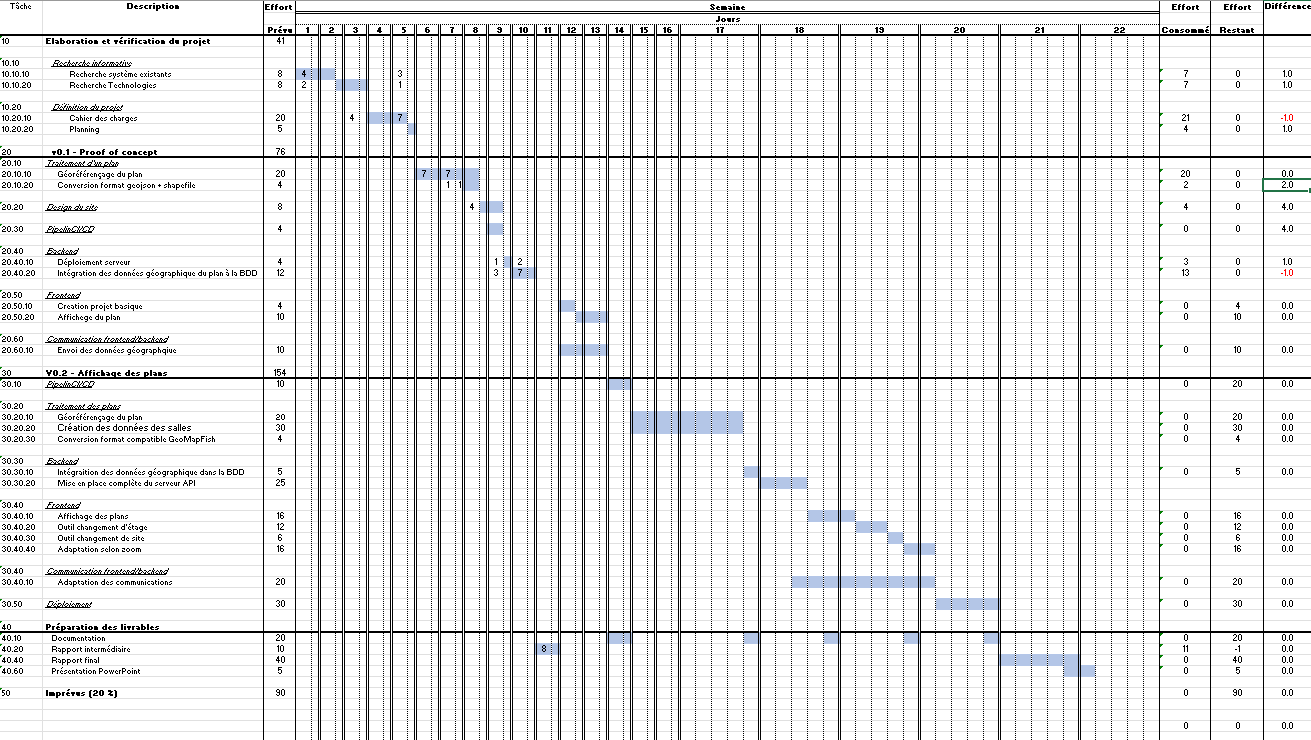
\includegraphics[scale=0.5]{planning.png}
\end{figure}

\section{Echéances et étapes}
Les principales échéances de ce travail sont le rendu d'un cahier des charges le jeudi 14 avril 2022,
le rendu d'un rapport intermédiaire le lundi 16 mai 2022,
le rendu final du projet le vendredi 29 juillet 2022 et
finalement une défense qui aura lieu entre le 22 août et le 16 septembre.

En planifiant le projet, j'ai prévu deux grandes étapes :
une première version servant de proof of concept que je prévois de finir le dimanche 29 mai 2022
et une deuxième version qui sera la version final de mon projet pour le 29 juillet 2022.
Je décris ces versions dans les sections suivantes.
J'ai aussi planifié du temps pour documenter mon travail.

D'autres versions pourront être mis en place par la suite afin de rajouter des fonctionnalités,
mais cela demanderait plus de temps que ce qui a été planifié pour le TB.

\section{Elaboration du projet}
Afin de commencer le projet, il me fallait acquérir des connaissances sur les applications webGIS.
C'est pourquoi j'ai planifié 16 heures dans cette recherche de connaissances.

J'ai aussi prévu 25 heures pour la rédaction du cahier des charges et du planning.

\section{Première version du projet}
La première étape, était la prise en main des différentes technologies afin de vérifier la faisabilité du projet.
Le but est de mettre en place une application web minimaliste, n'affichant qu'un étage avec ses salles et n'offrant pas de fonctionnalités supplémentaires.

Je me suis fixé pour la réaliser 7 semaines de travail :
24 heures serait consacrées au traitement d'un plan d'un seul étage,
8 heures pour le design de l'application,
4 heures pour la mise en place d'un pipeline CI/CD,
16 heures pour stocker les données dans la base de données et installer un serveur api basique,
et finalement 24 heures pour m'occuper du frontend et de la communication entre le frontend et le backend.

\section{Deuxième version du projet}
Le deuxième étape est la mise en place de la solution finale pour ce travail.
J'y consacrerai 10 heures pour l'amélioration du pipeline CI/CD,
54 heures pour le traitement des plans de tous les étages du site de Cheseaux,
30 heures pour la mise en place du serveur API et de la base de données,
70 heures pour la mise en place du frontend et des fonctionnalités comme le changement d'étages
et finalement 30 heures pour déployer l'application sur une machine virtuelle de la HEIG-VD.

\section{Documentation du travail}
La documentation du travail étant importante, j'ai aussi planifié celle-ci:
J'ai prévu de consacrer 20 heures à la documentation du code et du repository git,
10 heures pour le rapport intermédiaire,
40 heures pour le rapport final du travail,
et finalement 5 heures pour la conception d'une présentation pour la défense du projet.

\section{Différences entre planning et réalité}
A l'écriture de ce rapport, je suis encore à la première étape du projet.
Pour l'instant, j'ai nécessité moins de travail que planifié.
Cela est dû au fait que j'ai été un peu pessimiste sur certaines tâches,
comme le traitement d'un plan ou la mise en place du serveur API.

J'ai aussi passé 2 heures de moins sur la recherche en début de projet,
car j'avais pris du retard dans la rédaction de mon cahier des charges et de mon planning.

Une tâche où j'ai gagné beaucoup de temps est le design du site. Je n'y ai passé que 4 heures au lieu de 8.
J'ai préféré pour cette tâche plutôt conceptualiser l'aspect des fonctionnalités
pour savoir dans quelle direction je voulais aller plutôt que créer un design précis.

Une tâche que je n'ai pas effectué est la mise en place du pipeline CI/CD, Ceci m'as fait gagné 4 heures.
Je n'avais pas encore assez de connaissance sur les technologies que j'utiliserais pour la mettre en place.
Je préfère l'effectuer à la fin de la première version, quand j'aurais une idée bien plus claire.

Une tâche qui m'a pris plus de temps que prévu est la rédaction du rapport que vous êtes en train de lire :
Initialement prévu à 10 heures de travail celui-ci me prendra entre 13 à 18 heures pour être complétés.

\chapter{Design de la solution}
Cette section décrit les designs que j'ai imaginé pour le site.
N'étant pas graphiste, ceux-ci ne sont pas précis et seront susceptible de changer lors de l'implémentation.
De plus, des outils comme le menu de filtrage ou la recherche risque de ne pas être implémenté.

\section{Design global}

\begin{figure}[H]
    \caption{Design global}
    \centering
    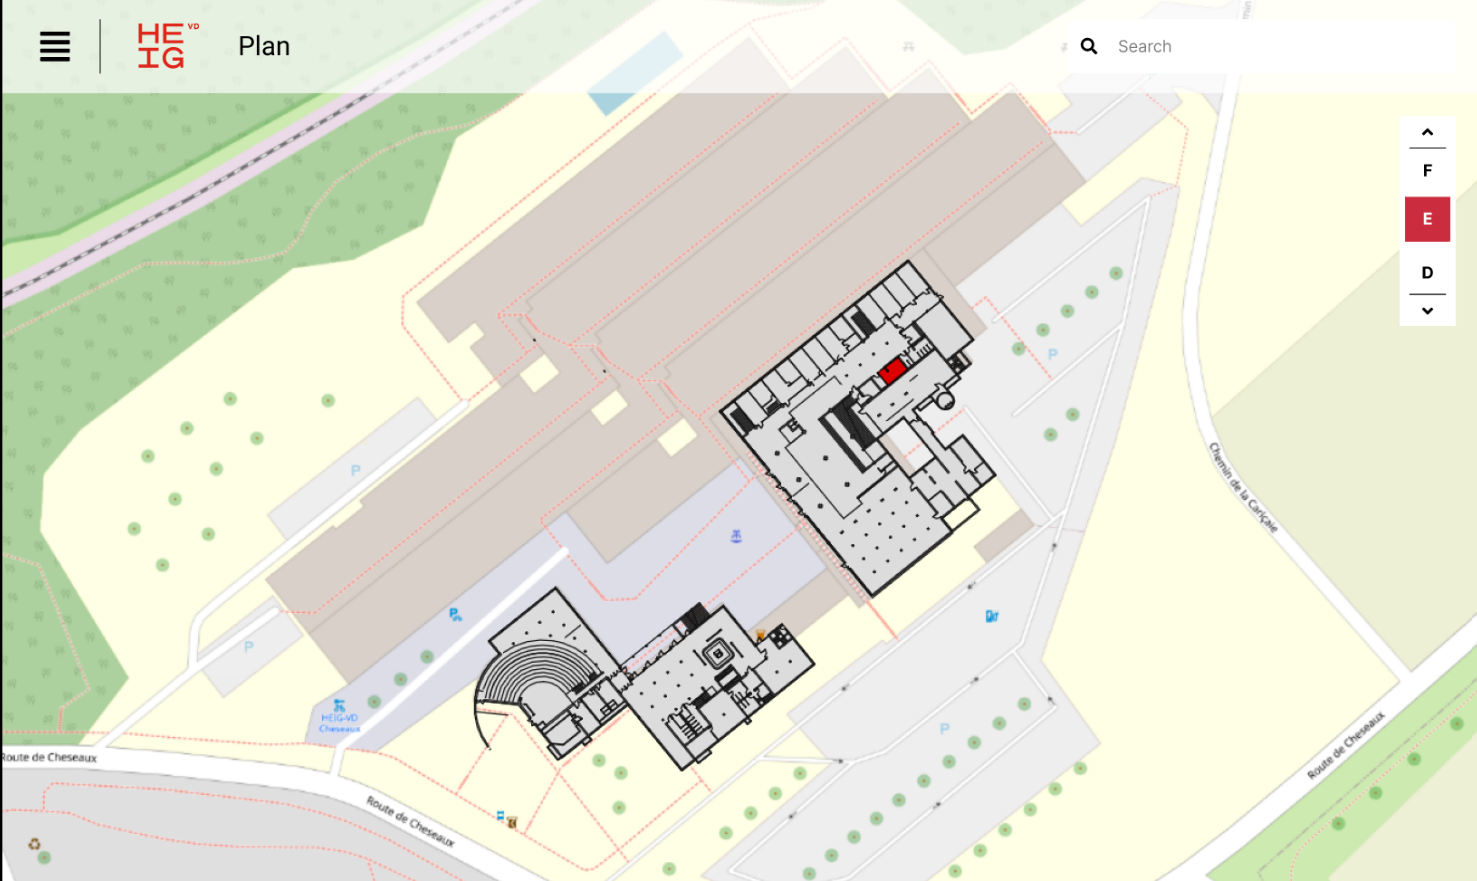
\includegraphics[scale=0.4]{designGlobal.png}
\end{figure}

L'aspect global essaie de respecter la charte graphique du site heig-vd.ch/ en utilisant son logo, son code couleur et la transparence du header.
Le design a été conçu pour un écran au format 16/9, mais l'application sera aussi disponible pour d'autre types d'écrans.
L'application sera sur une seule page sans scroll principal
(Des scrolls secondaire seront possibles pour des fonctionnalités comme la fenêtre d'informations).

Sur cette page on peut accéder à plusieurs outils :

\begin{itemize}
    \item Un menu pour filtrer les informations à afficher en cliquant sur le bouton en haut à gauche.
    \item Un outil de recherche à droite du header
    \item Un outil de changement d'étage à droite de la fenêtre
    \item Une fenêtre d'information en cliquant sur une salle ou en ayant effectué une recherche
\end{itemize}

\section{Outil de changement d'étage}

\begin{figure}[H]
    \caption{Design de l'outil de changement d'étage}
    \centering
    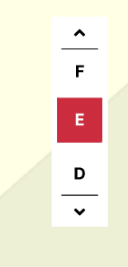
\includegraphics[scale=1]{designChangementEtage.png}
\end{figure}

L'outil de changement d'étage permet de modifier l'étage affiché sur le plan.
Il indique, en blanc sur fond rouge, l'étage actuel auquel se trouve l'utilisateur.
On pourra modifier celui-ci en cliquant sur les flèches.
L'outil indique aussi l'étage précédent et suivant
afin d'éviter que l'utilisateur ne sache pas sur quelle flèche cliquer pour accéder à l'étage désiré.

\section{Fenêtre d'informations}

\begin{figure}[H]
    \caption{Design de la fenêtre d'information}
    \centering
    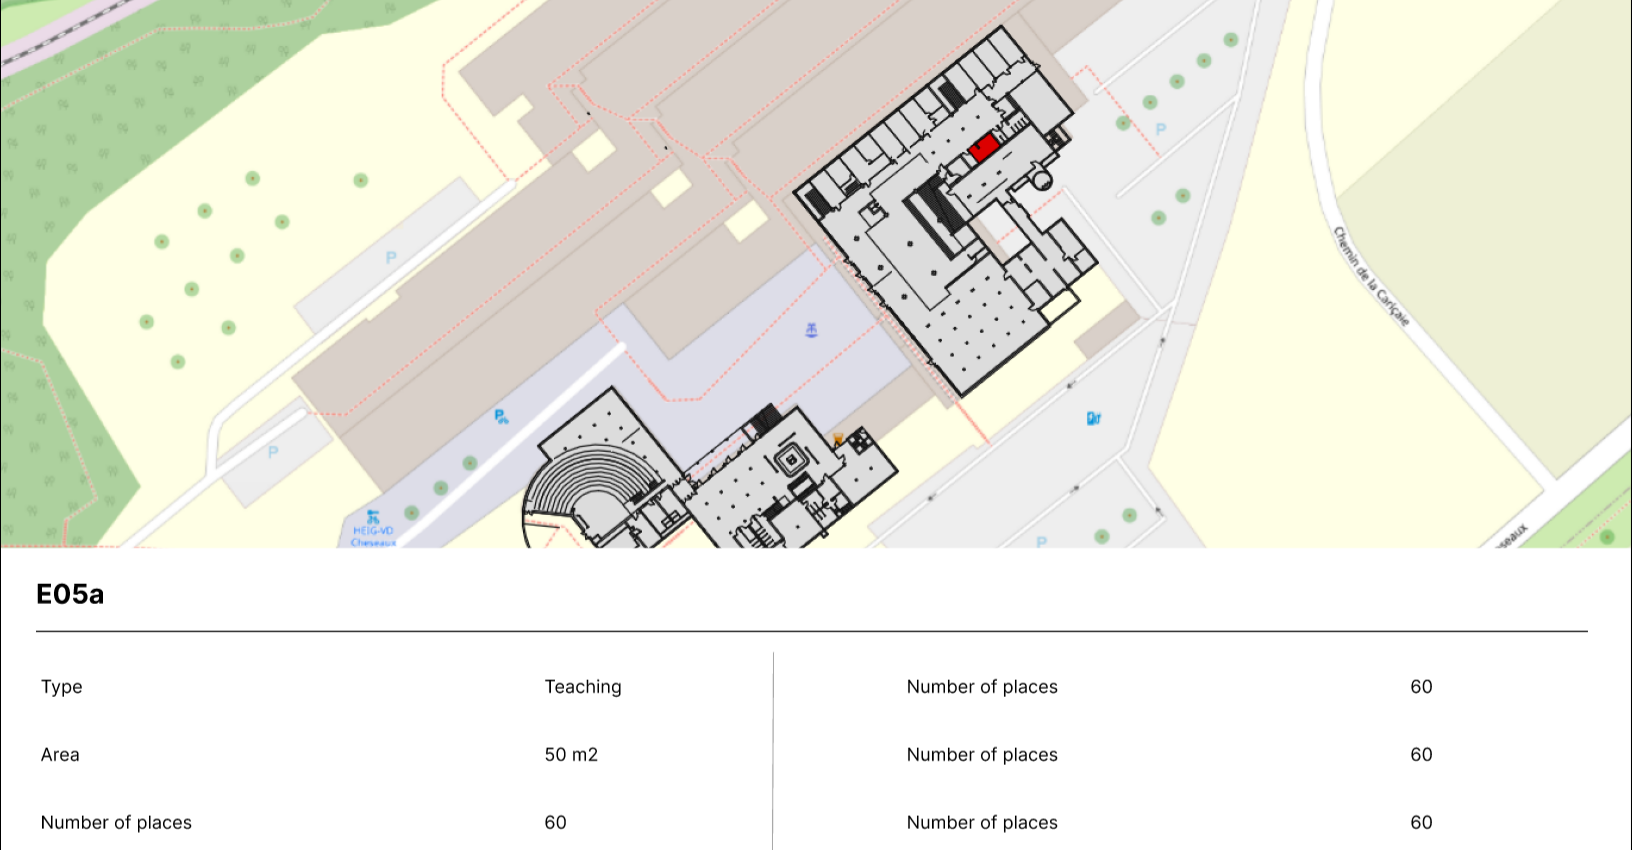
\includegraphics[scale=0.4]{designInfo.png}
\end{figure}

La fenêtre d'informations s'affichera sur le bas, lors d'un clic sur une salle ou après avoir exécuté une recherche.
Elle présentera les informations concernant la salle.
Pour la fermer, l'utilisateur pourra cliquer en dehors de la fenêtre.

\section{Menu de filtrage}

\begin{figure}[H]
    \caption{Design du menu de filtrage}
    \centering
    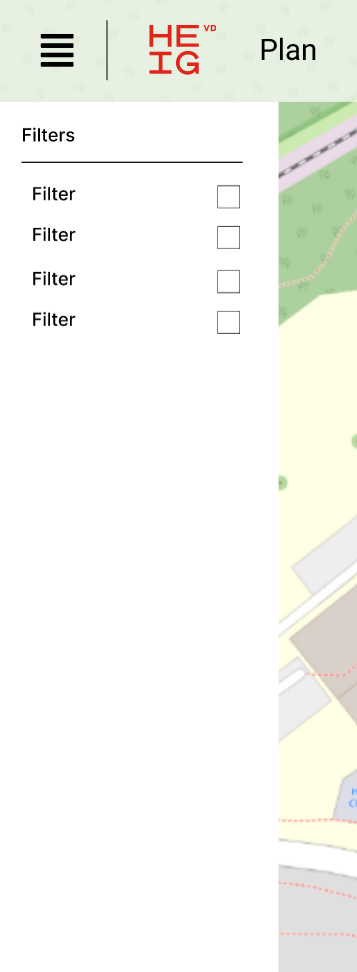
\includegraphics[scale=0.5]{designFilter.png}
\end{figure}

Le menu de filtrage s'affichera sur la gauche de l'écran, lorsque l'utilisateur cliquera sur le bouton en haut à droite.
Elle permettra d'ajouter ou enlever des éléments à afficher sur la carte.
Pour sortir du menu, l'utilisateur pourra cliquer en dehors de celui-ci, ou à nouveau sur le bouton.

\section{Outil de recherche}

\begin{figure}[H]
    \caption{Design de l'outil de recherche}
    \centering
    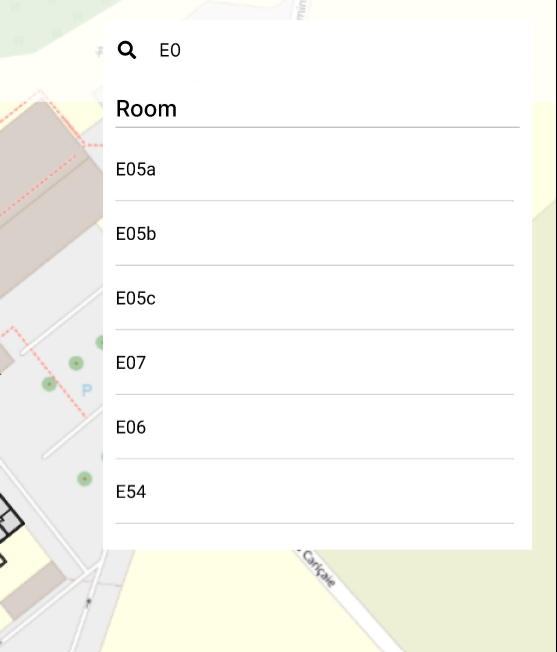
\includegraphics[scale=0.5]{designRecherche.png}
\end{figure}

Lorsque l'utilisateur commencera à taper des caractères dans le formulaire de recherche celui ci proposera un menu de suggestions.
Si l'utilisateur clique sut la touche entrée ou sur une des suggestions, l'affichage du plan se modifiera pour afficher la ressource demandé.

\chapter{Création des données géographiques}

\section{Les plans}
Pour ce projet on m'a fourni les plans de la HEIG-VD pour les sites de Cheseaux et de St-Roch.
Cependant, les plans étaient dans un système de coordonnées local.
Afin les projeter dans un autre système il fallait les géoréférencer aux bonnes coordonnées.

La première étape de mon travail de bachelor était donc de traiter ces plans et d'en extraire les données géographiques comme le contour de chaque salle.
Pour y'arriver, M. Ingensand m'a conseillé d'utiliser le logiciel QGIS.

\section{Géoréférencement des plans dans QGIS}
\begin{figure}[H]
    \caption{Résultat final du géoréférencement d'un plan}
    \centering
    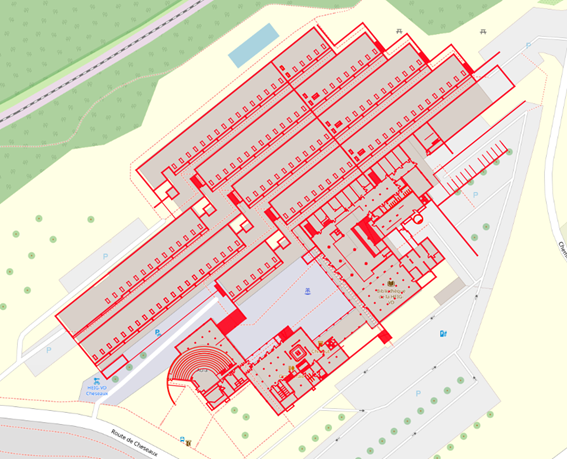
\includegraphics{Géoréférencement.png}
\end{figure}

Avant même d'ouvrir le logiciel, il faut choisir la projection (système de coordonnées ) dans laquelle les plans seront géoréférencé.
J'ai choisi la norme ESPG : 3857 - WGS 84 / Pseudo-Mercator, car c'est celle utilisé par open street map.
Cela me simplifiera la vie dans l'implémentation de l'application web.

Dans une première étape, j'ai d'abord sélectionné les calques contenant les informations utiles,
puis importer ceux-ci grâce à l'outil intégré dans QGIS "Import Layers from DWG/DXF "

La deuxième étape était le géoréférencement.
Pour ce faire, j'ai intégré le fond de carte Open Street Map qui servira de référence pour le placement des calques.
Ensuite, grâce au plugin " Vector Bender " j'ai effectué une transformation affine sur les plans, afin de les déplacer vers ma référence.
Finalement j'ai enregistré ceux-ci dans le format " ESRI shapefile " qui est plus adapté pour les manipulations dans ce logiciel.

\section{Création des informations géographiques}
\begin{figure}[H]
    \caption{Résultat final de la création d'informations d'un plan}
    \centering
    \includegraphics{créatioNgeodata.png}
\end{figure}

Dans une deuxième étape, j'ai dû créer certaines informations, comme le contour des salles et des bâtiments.
Pour ce faire, j'ai créé pour chaque salle un calque vectorielle prenant des polygones,
dessiné les contours des salles en me référant au plan préalablement géoréférencé,
et enfin les exporter dans les formats " ESRI shapefile " et " geojson ".
J'ai aussi retravaillé les calques initiaux afin d'obtenir seulement les contours des bâtiments

\section{Problèmes rencontrés}
Le premier problème que j'ai rencontré était que lors de mes recherches de solutions pour le géoréférencement,
il a été dur de trouver de la documentation à jour pour QGIS.

Un second a été que Le plugin "Vector Bender" nécessite que tous les calques utilisés pour la transformation affine utilise la même projection.

\section{Tests}
\begin{figure}[H]
    \caption{Rendu de l'affichage de tests}
    \centering
    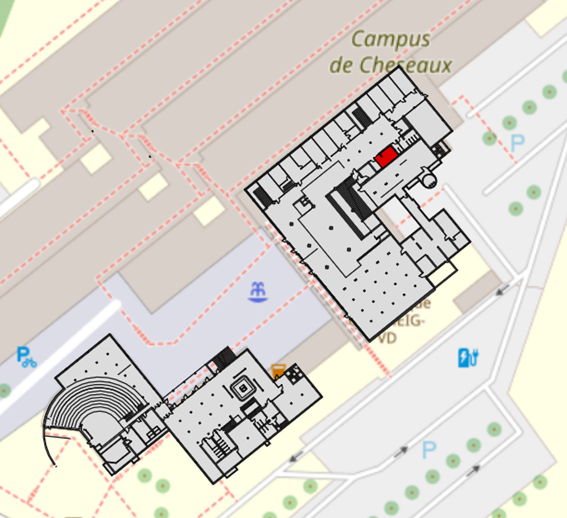
\includegraphics{TestsData.png}
\end{figure}

Afin de tester le géoréférencement des différents fichiers obtenus lors de la création des informations géographiques,
j'ai créé un petit prototype intégrant une version de base de l'api "Openlayers".
J'ai intégré dans celui-ci le fond de carte Open street map et rajouter différents calques intégrant les informations contenus dans les fichiers " geojson ".

\section{Base de données}

Dans ce chapitre, je vous présente la prise en main des technologies,
la modélisation de la base de données et comment je compte mettre en production une base de données.
Les codes sources pour le script d'insertion des données dans la base de données,
se trouve sur le repository github : https://github.com/Klab93/TB-PlanHeig/tree/main/dbCreator

\section{Prise en main}
La première étape de la création de la base de données relationnelle,
a été de prendre en main la technologie PostGreSQL et de l'extension PostGis.

J'avais initialement l'intention d'utiliser la technologie c2cgeoportal qui intègre Postgres et PostGis,
mais celle-ci m'as posé plusieurs problèmes:

\begin{itemize}
    \item La marche à suivre ne proposait que des commandes pour des utilisateurs de l'os GNU/Linux. Il m'aurait fallu installer l'os et le configurer, ce qui m'aurait fait perdre beaucoup de temps.
    \item Il n'y avait pas beaucoup de documentation pour résoudre d'éventuelle problème.
    \item Cette solution était trop complète pour les besoins que j'avais.
    \item J'allais perdre énormément de temps dessus alors que je mets en place un système peu compliqué.
\end{itemize}

Pour toutes ces raisons, j'ai préféré implémenter ma solution personnelle.
J'ai d'abord essayer d'intégrer des informations géographiques dans Postgres à l'aide de différents outils que proposent pgAdmin 4,
l'interface graphique permettant de gérer les base de données PostGreSQL.

La dernière étape de la prise en main était d'analyser comment faisait PostGis pour intégrer ces données.
Il s'avéra qu'elles étaient stockées dans une seule colonne sous forme d'une chaine de caractères en hexadécimal.

\section{Modélisation}
La deuxième étape a été de modéliser la base de données en créant le schéma ci-dessous en notation UML.
\figi{DB_model.xml}{12cm}{Modèle de la base de donnée relationnelle}

La base de données sera composé des six tables suivantes :

La table building représente les différents sites de la HEIG-VD. Elle est composée des champs id
et name et d'un champ geometry qui sera utile pour afficher la structure du site lors d'un zoom éloigné.
Une relation 1 à plusieurs la relie à la table Floor.

La table Floor représente les différents étages d'un site. Elle est composée des champs id et name.
Deux relations 1 à plusieurs la relie aux tables Floor geometry et Room.

La table Floor geometry est nécessaire car un étage est représenté par plusieurs données géométriques.
Cette table est composée des champs id et geometry ainsi que type (le type de géometrie stocké).
Deux types sont stockés dans cette table : des multipolygon et des multiline.
Ce champ permet de les distinguer lors de l'affichage côté frontend.

La table room représente les salles d'un site.
Elle est composé id, name, area (la surface de la salle), type (le type de salle par exemple une salle de cours) et geometry.

Les deux dernière tables Equipment et Person représentent des ressources et leurs informations. Elles sont rattachées à une salle.
Les différents champs sont susceptibles de changer lors de l'implémentation.

\section{Création de la base de données}
Afin d'éviter de stocker toutes mes données à la main dans la base de données,
j'ai écris un script en Node Js qui se connecte à la base de données, crée les tables,
lis les fichiers en geojson contenant les informations géographiques,
et insère celle-ci dans la base de données.

Ce script utilise la librairie "pg" qui permet facilement de se connecter à la base de données et d'exécuter des requêtes.
Pour l'instant il ne crée que quatre tables et n'y insère que les données géographiques de l'étage E.
Cela me permet de tester rapidement la première version de l'application web.

\section{Futur}
Dans la suite de ce projet, je traiterai les plans des autres étages.
Je générerai les données concernant les personnes et les ajouterai.
Pour le déploiement de la base de données, je mettrai en place un container docker directement sur la machine virtuelle.
J'adapterai le script pour qu'il envoie les données sur ce container.

\chapter{Backend }
Le serveur API s'occuper de récupérer les données depuis la base de données et de de les envoyer à l'application web.
Les codes sources du serveur API sont disponibles sur le repository github : https://github.com/Klab93/TB-PlanHeig/tree/main/serverAPI

\section{Première implémentation}
La première implémentation du serveur utilise le Framework web express JS.
Une application web peut lui faire 3 types de requêtes :
Récupérer les lignes formant les contours de l'étage E,
Récupérer les polygones formant le fond de l'étage E,
Récupérer les polygones de toutes les salles de l'étage E avec leurs noms.

A chacune de ses requêtes le serveur ira récupérer les données dans la base de données,
sous format geojson, à l'aide d'une requête SQL.
Par la suite il envoie directement ces données à l'application web.

\section{Future implémentation}
Par la suite, le serveur API subira une seconde implémentation.
J'utiliserai le Framework web Nest Js, car celui-ci est plus complet.
Les requêtes seront généralisées pour tous les étages,
et d'autres requêtes seront ajoutés pour offrir plus de fonctionnalités.


\chapter{Frontend}

\section{Stratégie de récolte des données géographiques}

\chapter{Conclusion}
Le projet est en bonne voie et la première version de l'application sera normalement fini dans 2 semaines.
Je n'ai encore pas eu de gros imprévus ou de grosses difficultés et j'arrive à suivre le planning que je m'étais fixé au début du projet.
Grâce à la préparation en amont du projet, j'ai des repères clairs du travail à accomplir par la suite.
Il me restera des points à éclaircir mais il n'y aura sûrement aucsun élément insurmontable.

\vfil
\hspace{8cm}\makeatletter\@author\makeatother\par
\hspace{8cm}\begin{minipage}{5cm}
    %%if
    % Place pour signature numérique
    \printsignature
    %%fi
\end{minipage}
\clearpage

\appendix
\appendixpage
\addappheadtotoc

\chapter{Planning}

\begin{figure}[H]
    \centering
    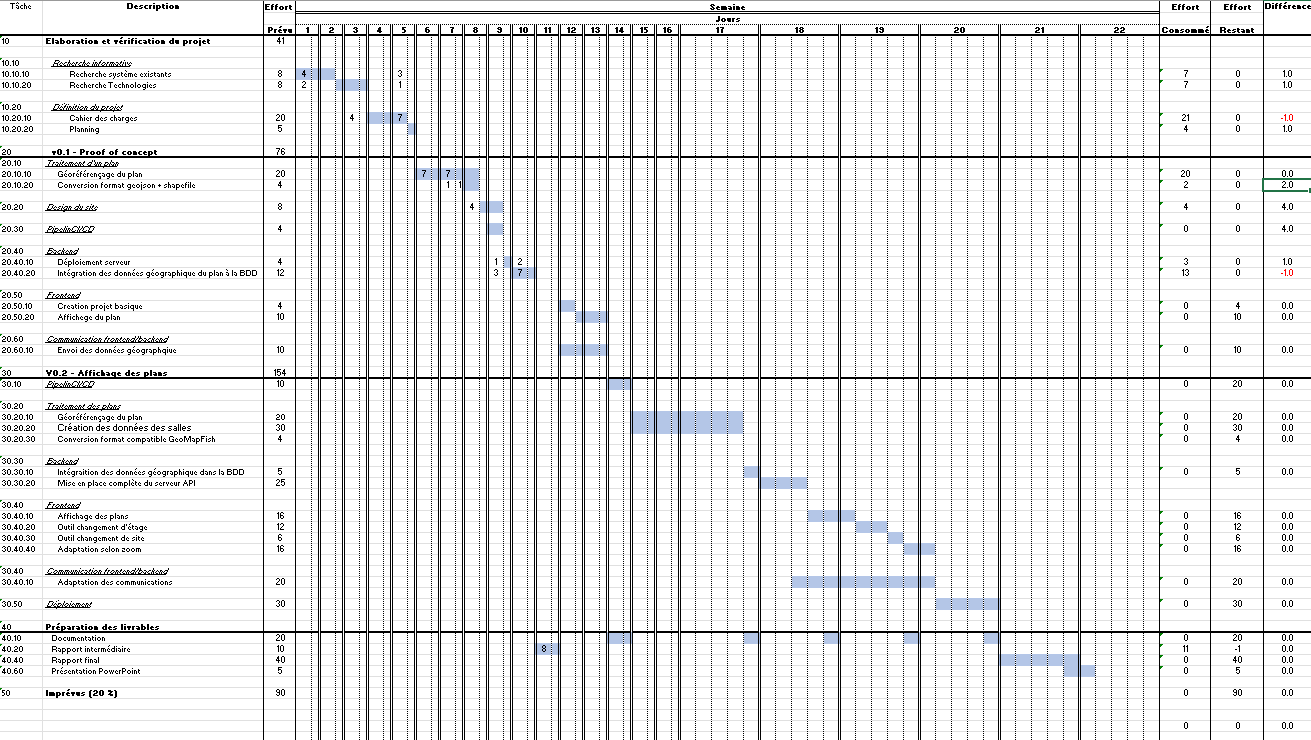
\includegraphics[scale=0.6, angle=90]{planning.png}
\end{figure}

\let\cleardoublepage\clearpage
\backmatter

\label{glossaire}
\printnoidxglossary
\printbibliography
\label{index}
\printindex

\end{document}
